\فصل{ارزیابی}

در این فصل به ارزیابی پروتکل پیشنهادی خود می‌پردازیم. همان‌طور که در فصل‌های قبل و به ویژه ~\ref{prevWorks} به آن اشاره شد، پروتکل NLSR قابل‌توجه‌ترین و جدیدترین پروتکل پیشنهادی مسیریابی در NDN است و به همین دلیل برای این ارزیابی، به مقایسه‌ی ویژگی‌های این پروتکل و پروتکل پیشنهادی خود می‌پردازیم.

یکی از ویژگی‌های مهم NDN پشتیبانی آن از چندمسیری در دامنه‌ی ارسال است و پروتکل‌های مسیریابی در این شبکه باید بتوانند تا حد ممکن از این قابلیت استفاده کنند. NLSR با چند بار اجرای الگوریتم کوتاه‌ترین مسیر روی گراف شبکه، برای هر پیشوند واسط‌های مسیریاب را به ترتیب فاصله‌ی آن‌ها از تولید‌کننده‌ی پیشوند رتبه‌بندی می‌کند. پروتکل پیشنهادی به دلیل مبتنی بودن بر بردار فاصله، می‌تواند همین کار را تنها با اجرای یک الگوریتم مرتب‌سازی روی اطلاعات کسب‌شده از بسته‌های DA از واسط‌های مختلف خود انجام دهد. بدین‌ترتیب سربار محاسبه‌ی مسیریاب کاهش چشمگیری خواهد داشت.

در مورد مسیریابی پیشوند‌ها، پروتکل NLSR و پروتکل پیشنهادی ما، عملکرد مشابهی دارند. در هر دو پروتکل، بسته‌های اعلام‌کننده‌ی پیشرفت با استفاده از پروتکل Sync در سرتاسر شبکه توزیع می‌شوند، زیرا برای مسریابی درست، تمام مسیریاب‌ها باید از تولیدکنندگان مختلف یک داده اطلاع داشته باشند. این امر به دلیل زیاد بودن داده‌ها برای شبکه سربار قابل‌توجهی تولید خواهد کرد ولی بدون چشم‌پوشی از بخشی از داده‌ها، از آن گریزی نیست. یکی از راه‌حل‌هایی که برای این مسئله به نظر می‌رسد استفاده از روشی مشابه \cite{two-layer} است که در آن داده‌هایی که درخواست کمتری دارند به کل شبکه توزیع نمی‌شود. یافتن راهی مناسب برای کم‌کردن این سربار از کارهای آینده‌ی ما خواهد بود.

تفاوت اصلی بین NLSR و پروتکل پیشنهادی ما در نحوه‌ی توزیع بسته‌های مربوط به مسیریابی بین مسیریاب‌هاست. از آن‌جایی که NLSR پروتکلی مبتنی بر وضعیت پیوند است، بسته‌های مربوط به این نوع مسیریابی نیز مشابه بسته‌های اعلام‌کننده‌ی پیشوندها در سرتاسر شبکه توزیع می‌شوند. این در حالی است که در پروتکل پیشنهادی ما که مبتنی بر بردار فاصله است، ارسال بسته‌های DA تنها در صورتی انجام می‌گیرد که بهترین مسیر یک مسیریاب با دریافت یک بسته‌ی DA  تغییر کند. از مقایسه‌ی این دو روش چنین بر می‌آید که تعداد بسته‌های ردوبدل شده‌ای که مربوط به مسیریابی بین مسیریاب‌ها هستند، در پروتکل پیشنهادی ما به مراتب کمتر از NLSR هستند. برای بررسی این امر با ساده‌کردن پروتکل‌ها به شبیه‌سازی آن‌ها روی دو شبکه پرداختیم. این ساده‌سازی از آن جهت صورت گرفته است که تنها بسته‌هایی برای ما اهمیت داشتند که مربوط به مسیریابی بین مسیریاب‌ها هستند، زیرا عملکرد دو پروتکل در مورد سایر بسته‌ها مشابه است. 

شبیه‌سازی با استفاده از زبان جاوا روی دو شبکه‌، یکی با شش مسیریاب و دیگری با ده مسیریاب انجام شده است. شبکه‌ی اول، همان شبکه‌ای است که برای ارزیابی NLSR مورد استفاده قرار گرفته است، و شبکه‌ی دوم با ده مسیریاب برای نشان دادن تاثیر افزایش اندازه‌ی شبکه بر مسیریابی طراحی شده است. برای هر شبیه‌سازی، دنباله‌ای از به‌روزرسانی هزینه‌ی پیوندها بر شبکه اعمال شده است و تعداد بسته‌های ردوبدل شده، به ازای هر پنج به‌روزرسانی، ثبت شده است. لازم به ذکر است که در شبکه‌ی اول هزینه‌ی تمام پیوندها در ابتدای کار یک در نظر گرفته شده است. هم‌چنین به دلیل این که هدف بررسی تعداد بسته‌های ردوبدل شده برای به‌روزرسانی یک شبکه است و نه راه‌اندازی آن، شبیه‌سازی بر روی شبکه در حالت پایدار آغاز شده است، بدین معنی که در ابتدا FIBها با اطلاعات لازم و صحیح پر شده‌اند و اعمال دنباله‌ی به‌روزرسانی پس از آن انجام گرفته است. هم‌چنین شبیه‌ساز پس از شروع هر به‌روزرسانی، تا پایدار شدن شبکه منتظر می‌ماند و سپس به‌روزرسانی بعدی را اعمال می‌کند. 

شکل ~\ref{fig:Net1} توپولوژی شبکه‌ی مورداستفاده در ارزیابی NLSR را نشان می‌دهد. این شبکه برای مقایسه‌ی دو پروتکل از نظر تعداد بسته‌های مربوط به مسیریابی بین مسیریاب‌ها مورد استفاده قرار گرفته است. شکل ~\ref{fig:Plot1} نمودار تغییر تعداد بسته‌ها برحسب تعداد به‌روزرسانی‌ها را در دو پروتکل نشان می‌دهد. \begin{figure}[h!]
\centering
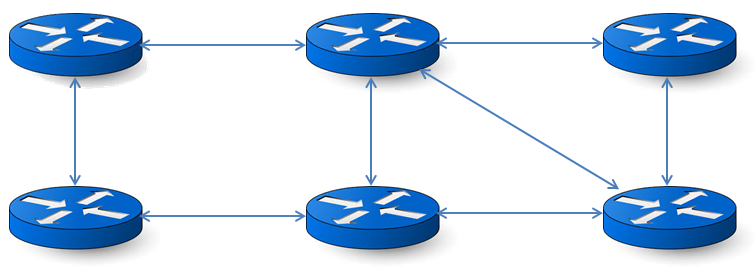
\includegraphics[scale=0.7]{./resources/figures/Network1.png}
%\makebox[\textwidth][c]{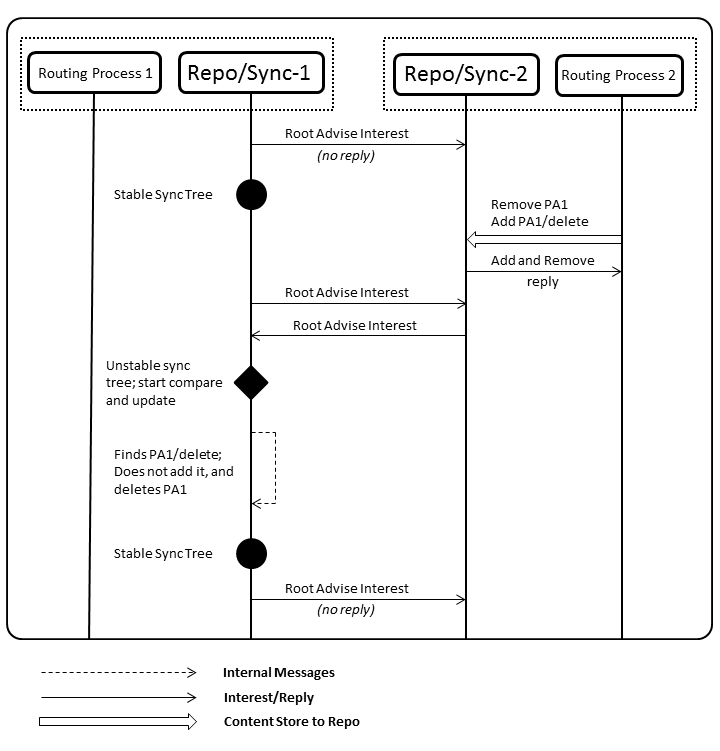
\includegraphics[width=1.1\textwidth]{./resources/figures/Sync2.png}}%
\caption{توپولوژی شبکه‌ی ۱ استفاده شده در شبیه‌سازی}
\label{fig:Net1}
\end{figure}
\begin{figure}[h!]
\centering
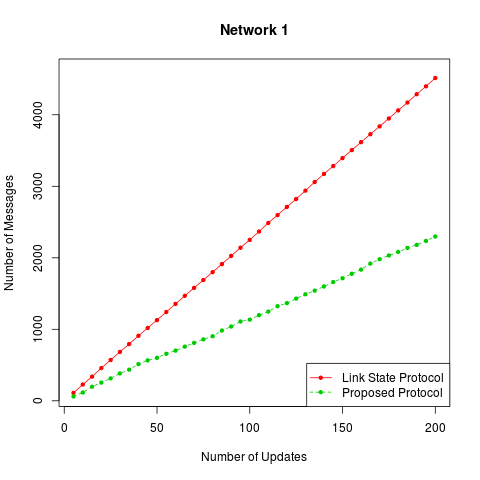
\includegraphics[scale=0.8]{./resources/figures/Test1.png}
%\makebox[\textwidth][c]{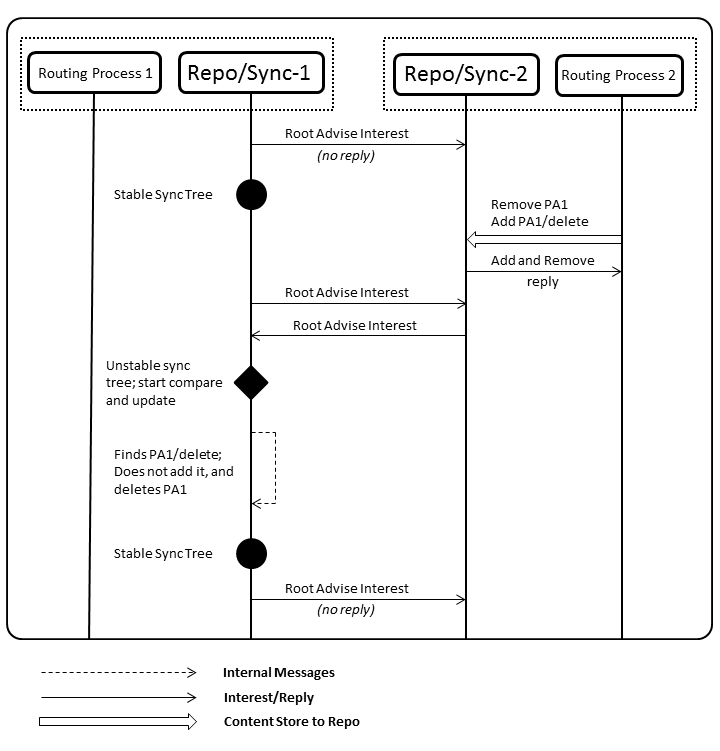
\includegraphics[width=1.1\textwidth]{./resources/figures/Sync2.png}}%
\caption{مقایسه‌ی تعداد بسته‌های ردوبدل شده برای مسیریابی بین مسریاب‌ها در پروتکل NLSR و پروتکل پیشنهادی ما}
\label{fig:Plot1}
\end{figure}همان‌طور که در نمودار مشخص است، تعداد بسته‌های ردوبدل شده در پروتکل مبتنی بر وضعیت پیوند به طور قابل‌توجهی بیشتر از پروتکل پیشنهادی ماست. هم‌چنین شیب دو منحنی نشان‌دهنده‌ی این است که افزایش تعداد به‌روزرسانی‌ها تاثیر بیشتری بر پروتکل مبنتی بر وضعیت پیوند دارد و همان‌طور که در شکل مشخص است، به تدریج فاصله‌ی بیشتری از منحنی پروتکل پیشنهادی پیدا می‌کند. نکته‌ی قابل توجه دیگر در این نمودار، خطی بودن منحنی پروتکل مبتنی بر وضعیت پیوند است که نشان‌گر این است که تعداد بسته‌های ردو‌بدل شده مستقل از به‌روزرسانی و تاثیر آن بر شبکه است. این در حالی است که در منحنی پروتکل پیشنهادی، با وجود داشتن شکل کلی خطی، تغییرات جزیی غیرخطی دیده می‌شود. این تغییرات نمایان‌گر این مسئله هستند که خود به‌روزرسانی نیز، هر چند ناچیز، بر تعداد بسته‌های ردوبدل شده تاثیر می‌گذارد. 

شکل ~\ref{fig:Net2} توپولوژی شبکه‌ی بزرگتری را نشان می‌دهد که برای مقایسه‌ی دو پروتکل مورد استفاده قرار گرفته است و شکل ~\ref{fig:Plot2} نتایج شبیه‌سازی روی ای شبکه را در نمودار به نمایش می‌گذارد. این نمودار نیز نتایج به دست آمده از شبیه‌سازی قبلی را مورد تایید قرار می‌دهد.

تفاوت دیگری که پروتکل پیشنهادی ما با NLSR دارد در نحوه‌ی استفاده از مخازن و پروتکل Sync در CCNx است. NLSR بدون تغییر از پروتکل Sync استفاده می‌کند. همان‌طور که پیش از این اشاره شد پروتکل Sync از حذف داده‌های یک مجموعه به درستی پیشتیبانی نمی‌کند. در پروتکل NLSR ، به دلیل استفاده از شماره‌ی نسخه در نام بسته‌ها این مسئله مشکل چندانی ایجاد نمی‌کند. هر بسته‌ی مسیریابی طول عمری دارد و هر مسیریاب مجموعه‌ی محلی خود را برای اطمینان از تمام نشدن طول عمر بسته‌ها بررسی می‌کند. در صورت تمام شدن عمر یک بسته، مسیریاب آن را از مجموعه‌ی محلی خود پاک می‌کند. به همین دلیل هر مسیریاب باید در بازه‌های مشخصی به بسته‌های قدیمی خود را با شماره‌ی نسخه‌ی جدیدتری در شبکه توزیع کند. این فرآیند سبب انتشار تعداد زیادی بسته در کنار بسته‌های فراوان مربوط به مسیریابی مبتنی بر وضعیت پیوند می‌شود و سربار زیادی برای شبکه به همراه خواهد داشت. ما در پروتکل پیشنهادی خود با اعمال تغییراتی در پروتکل Sync سعی بر پشتیبانی از حذف بسته‌ها از مجموعه‌های داده داشته‌ایم تا نیازی به فرستادن چندباره‌ی هر بسته و استفاده از شماره‌ی نسخه به وجود نیاید.

 \begin{figure}[h!]
\centering
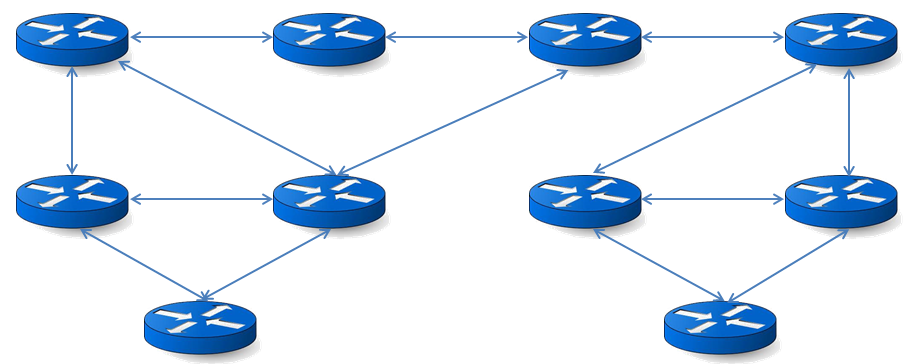
\includegraphics[scale=0.6]{./resources/figures/Network2.png}
%\makebox[\textwidth][c]{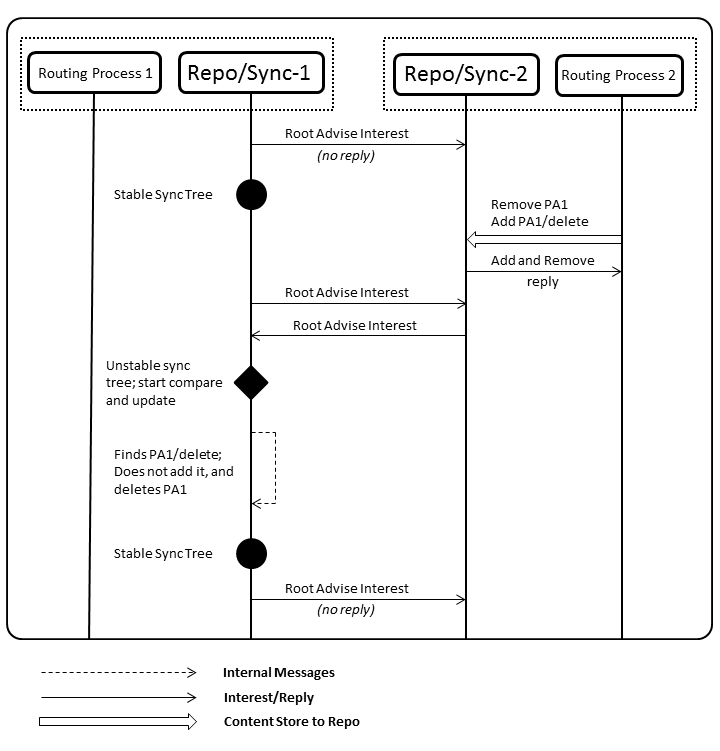
\includegraphics[width=1.1\textwidth]{./resources/figures/Sync2.png}}%
\caption{توپولوژی شبکه‌ی ۲ استفاده شده در شبیه‌سازی}
\label{fig:Net2}
\end{figure}

در مجموع با وجود این که پروتکل پیشنهادی ما در زمینه‌ی توزیع بسته‌های DA و نیز پشتیبانی از چندمسیری کارایی بهتری را نسبت به NLSR از خود نشان می‌دهد و در مورد توزیع پیشوندها عملکردی مشابه آن دارد، به دلیل مبتنی بودن بر بردار فاصله، همگرایی آن به نسبت پروتکل‌های مبتنی بر وضعیت پیوند دیرتر اتفاق می‌افتد. این امر به دلیل مشکلاتی هم‌چون شمارش بی‌انتهاست. همان‌طور که پیش از این به آن اشاره شد، روش‌هایی مانند سم معکوس برای کم‌کردن اثر این مشکل وجود دارد، هم‌چنین پروتکل‌های مبتنی بر بردار فاصله‌ای در شبکه‌های مبتنی بر IP به وجود آمده‌اند که به طور کامل این مشکل را برطرف کرده‌اند. ولی پیچیدگی اضافه‌شده به آن‌ها در کنار توجه به این مسئله که ظرفیت شبکه‌ی کنونی برای اجرای پروتکل‌های مبتنی بر وضعیت پبوند که به مراتب ساده‌تر هستند، سبب شده است استفاده از پروتکل‌های مبتنی بر فاصله به شبکه‌های کوچک‌تر محدود شود. با این توضیحات به نظر می‌رسد پروتکل پیشنهادی ما نیز، به دلیل وضعیت مشابه، برای استفاده در شبکه‌های کوچک‌تر مناسب‌تر باشد.
\begin{figure}[h!]
\centering
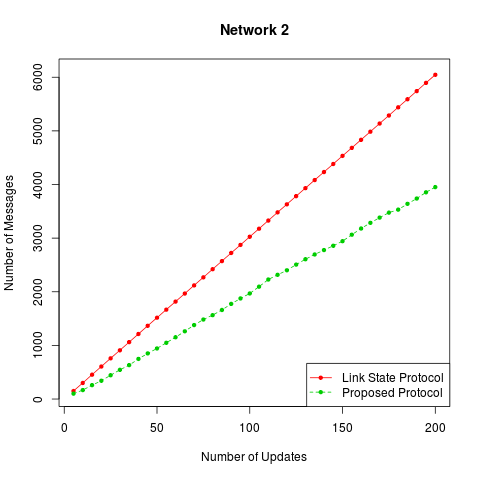
\includegraphics[scale=0.7]{./resources/figures/Test2.png}
%\makebox[\textwidth][c]{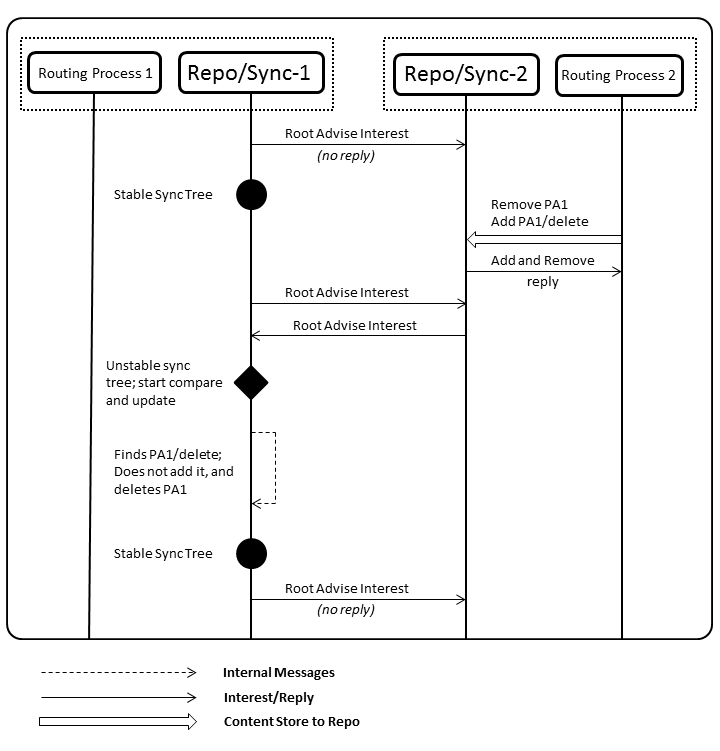
\includegraphics[width=1.1\textwidth]{./resources/figures/Sync2.png}}%
\caption{مقایسه‌ی تعداد بسته‌های ردوبدل شده برای مسیریابی بین مسریاب‌ها در پروتکل NLSR و پروتکل پیشنهادی ما}
\label{fig:Plot2}
\end{figure}


